
%% bare_jrnl_transmag.tex
%% V1.4a
%% 2014/09/17
%% by Michael Shell
%% see http://www.michaelshell.org/
%% for current contact information.
%%
%% This is a skeleton file demonstrating the use of IEEEtran.cls
%% (requires IEEEtran.cls version 1.8a or later) with an IEEE 
%% Transactions on Magnetics journal paper.
%%
%% Support sites:
%% http://www.michaelshell.org/tex/ieeetran/
%% http://www.ctan.org/tex-archive/macros/latex/contrib/IEEEtran/
%% and
%% http://www.ieee.org/

%%*************************************************************************
%% Legal Notice:
%% This code is offered as-is without any warranty either expressed or
%% implied; without even the implied warranty of MERCHANTABILITY or
%% FITNESS FOR A PARTICULAR PURPOSE! 
%% User assumes all risk.
%% In no event shall IEEE or any contributor to this code be liable for
%% any damages or losses, including, but not limited to, incidental,
%% consequential, or any other damages, resulting from the use or misuse
%% of any information contained here.
%%
%% All comments are the opinions of their respective authors and are not
%% necessarily endorsed by the IEEE.
%%
%% This work is distributed under the LaTeX Project Public License (LPPL)
%% ( http://www.latex-project.org/ ) version 1.3, and may be freely used,
%% distributed and modified. A copy of the LPPL, version 1.3, is included
%% in the base LaTeX documentation of all distributions of LaTeX released
%% 2003/12/01 or later.
%% Retain all contribution notices and credits.
%% ** Modified files should be clearly indicated as such, including  **
%% ** renaming them and changing author support contact information. **
%%
%% File list of work: IEEEtran.cls, IEEEtran_HOWTO.pdf, bare_adv.tex,
%%                    bare_conf.tex, bare_jrnl.tex, bare_conf_compsoc.tex,
%%                    bare_jrnl_compsoc.tex, bare_jrnl_transmag.tex
%%*************************************************************************


% *** Authors should verify (and, if needed, correct) their LaTeX system  ***
% *** with the testflow diagnostic prior to trusting their LaTeX platform ***
% *** with production work. IEEE's font choices and paper sizes can       ***
% *** trigger bugs that do not appear when using other class files.       ***                          ***
% The testflow support page is at:
% http://www.michaelshell.org/tex/testflow/



\documentclass[journal,transmag,twoside]{IEEEtran}
%
% If IEEEtran.cls has not been installed into the LaTeX system files,
% manually specify the path to it like:
% \documentclass[journal]{../sty/IEEEtran}





% Some very useful LaTeX packages include:
% (uncomment the ones you want to load)


% *** MISC UTILITY PACKAGES ***
%
%\usepackage{ifpdf}
% Heiko Oberdiek's ifpdf.sty is very useful if you need conditional
% compilation based on whether the output is pdf or dvi.
% usage:
% \ifpdf
%   % pdf code
% \else
%   % dvi code
% \fi
% The latest version of ifpdf.sty can be obtained from:
% http://www.ctan.org/tex-archive/macros/latex/contrib/oberdiek/
% Also, note that IEEEtran.cls V1.7 and later provides a builtin
% \ifCLASSINFOpdf conditional that works the same way.
% When switching from latex to pdflatex and vice-versa, the compiler may
% have to be run twice to clear warning/error messages.






% *** CITATION PACKAGES ***
%
%\usepackage{cite}
% cite.sty was written by Donald Arseneau
% V1.6 and later of IEEEtran pre-defines the format of the cite.sty package
% \cite{} output to follow that of IEEE. Loading the cite package will
% result in citation numbers being automatically sorted and properly
% "compressed/ranged". e.g., [1], [9], [2], [7], [5], [6] without using
% cite.sty will become [1], [2], [5]--[7], [9] using cite.sty. cite.sty's
% \cite will automatically add leading space, if needed. Use cite.sty's
% noadjust option (cite.sty V3.8 and later) if you want to turn this off
% such as if a citation ever needs to be enclosed in parenthesis.
% cite.sty is already installed on most LaTeX systems. Be sure and use
% version 5.0 (2009-03-20) and later if using hyperref.sty.
% The latest version can be obtained at:
% http://www.ctan.org/tex-archive/macros/latex/contrib/cite/
% The documentation is contained in the cite.sty file itself.






% *** GRAPHICS RELATED PACKAGES ***
%
\ifCLASSINFOpdf
  \usepackage[pdftex]{graphicx}
  % declare the path(s) where your graphic files are
  % \graphicspath{{../pdf/}{../jpeg/}}
  % and their extensions so you won't have to specify these with
  % every instance of \includegraphics
  % \DeclareGraphicsExtensions{.pdf,.jpeg,.png}
\else
  % or other class option (dvipsone, dvipdf, if not using dvips). graphicx
  % will default to the driver specified in the system graphics.cfg if no
  % driver is specified.
  % \usepackage[dvips]{graphicx}
  % declare the path(s) where your graphic files are
  % \graphicspath{{../eps/}}
  % and their extensions so you won't have to specify these with
  % every instance of \includegraphics
  % \DeclareGraphicsExtensions{.eps}
\fi
% graphicx was written by David Carlisle and Sebastian Rahtz. It is
% required if you want graphics, photos, etc. graphicx.sty is already
% installed on most LaTeX systems. The latest version and documentation
% can be obtained at: 
% http://www.ctan.org/tex-archive/macros/latex/required/graphics/
% Another good source of documentation is "Using Imported Graphics in
% LaTeX2e" by Keith Reckdahl which can be found at:
% http://www.ctan.org/tex-archive/info/epslatex/
%
% latex, and pdflatex in dvi mode, support graphics in encapsulated
% postscript (.eps) format. pdflatex in pdf mode supports graphics
% in .pdf, .jpeg, .png and .mps (metapost) formats. Users should ensure
% that all non-photo figures use a vector format (.eps, .pdf, .mps) and
% not a bitmapped formats (.jpeg, .png). IEEE frowns on bitmapped formats
% which can result in "jaggedy"/blurry rendering of lines and letters as
% well as large increases in file sizes.
%
% You can find documentation about the pdfTeX application at:
% http://www.tug.org/applications/pdftex




% *** MATH PACKAGES ***
%
%\usepackage[cmex10]{amsmath}
% A popular package from the American Mathematical Society that provides
% many useful and powerful commands for dealing with mathematics. If using
% it, be sure to load this package with the cmex10 option to ensure that
% only type 1 fonts will utilized at all point sizes. Without this option,
% it is possible that some math symbols, particularly those within
% footnotes, will be rendered in bitmap form which will result in a
% document that can not be IEEE Xplore compliant!
%
% Also, note that the amsmath package sets \interdisplaylinepenalty to 10000
% thus preventing page breaks from occurring within multiline equations. Use:
%\interdisplaylinepenalty=2500
% after loading amsmath to restore such page breaks as IEEEtran.cls normally
% does. amsmath.sty is already installed on most LaTeX systems. The latest
% version and documentation can be obtained at:
% http://www.ctan.org/tex-archive/macros/latex/required/amslatex/math/





% *** SPECIALIZED LIST PACKAGES ***
%
%\usepackage{algorithmic}
% algorithmic.sty was written by Peter Williams and Rogerio Brito.
% This package provides an algorithmic environment fo describing algorithms.
% You can use the algorithmic environment in-text or within a figure
% environment to provide for a floating algorithm. Do NOT use the algorithm
% floating environment provided by algorithm.sty (by the same authors) or
% algorithm2e.sty (by Christophe Fiorio) as IEEE does not use dedicated
% algorithm float types and packages that provide these will not provide
% correct IEEE style captions. The latest version and documentation of
% algorithmic.sty can be obtained at:
% http://www.ctan.org/tex-archive/macros/latex/contrib/algorithms/
% There is also a support site at:
% http://algorithms.berlios.de/index.html
% Also of interest may be the (relatively newer and more customizable)
% algorithmicx.sty package by Szasz Janos:
% http://www.ctan.org/tex-archive/macros/latex/contrib/algorithmicx/




% *** ALIGNMENT PACKAGES ***
%
%\usepackage{array}
% Frank Mittelbach's and David Carlisle's array.sty patches and improves
% the standard LaTeX2e array and tabular environments to provide better
% appearance and additional user controls. As the default LaTeX2e table
% generation code is lacking to the point of almost being broken with
% respect to the quality of the end results, all users are strongly
% advised to use an enhanced (at the very least that provided by array.sty)
% set of table tools. array.sty is already installed on most systems. The
% latest version and documentation can be obtained at:
% http://www.ctan.org/tex-archive/macros/latex/required/tools/


% IEEEtran contains the IEEEeqnarray family of commands that can be used to
% generate multiline equations as well as matrices, tables, etc., of high
% quality.




% *** SUBFIGURE PACKAGES ***
%\ifCLASSOPTIONcompsoc
%  \usepackage[caption=false,font=normalsize,labelfont=sf,textfont=sf]{subfig}
%\else
%  \usepackage[caption=false,font=footnotesize]{subfig}
%\fi
% subfig.sty, written by Steven Douglas Cochran, is the modern replacement
% for subfigure.sty, the latter of which is no longer maintained and is
% incompatible with some LaTeX packages including fixltx2e. However,
% subfig.sty requires and automatically loads Axel Sommerfeldt's caption.sty
% which will override IEEEtran.cls' handling of captions and this will result
% in non-IEEE style figure/table captions. To prevent this problem, be sure
% and invoke subfig.sty's "caption=false" package option (available since
% subfig.sty version 1.3, 2005/06/28) as this is will preserve IEEEtran.cls
% handling of captions.
% Note that the Computer Society format requires a larger sans serif font
% than the serif footnote size font used in traditional IEEE formatting
% and thus the need to invoke different subfig.sty package options depending
% on whether compsoc mode has been enabled.
%
% The latest version and documentation of subfig.sty can be obtained at:
% http://www.ctan.org/tex-archive/macros/latex/contrib/subfig/



% *** FLOAT PACKAGES ***
%
%\usepackage{fixltx2e}
% fixltx2e, the successor to the earlier fix2col.sty, was written by
% Frank Mittelbach and David Carlisle. This package corrects a few problems
% in the LaTeX2e kernel, the most notable of which is that in current
% LaTeX2e releases, the ordering of single and double column floats is not
% guaranteed to be preserved. Thus, an unpatched LaTeX2e can allow a
% single column figure to be placed prior to an earlier double column
% figure. The latest version and documentation can be found at:
% http://www.ctan.org/tex-archive/macros/latex/base/


%\usepackage{stfloats}
% stfloats.sty was written by Sigitas Tolusis. This package gives LaTeX2e
% the ability to do double column floats at the bottom of the page as well
% as the top. (e.g., "\begin{figure*}[!b]" is not normally possible in
% LaTeX2e). It also provides a command:
%\fnbelowfloat
% to enable the placement of footnotes below bottom floats (the standard
% LaTeX2e kernel puts them above bottom floats). This is an invasive package
% which rewrites many portions of the LaTeX2e float routines. It may not work
% with other packages that modify the LaTeX2e float routines. The latest
% version and documentation can be obtained at:
% http://www.ctan.org/tex-archive/macros/latex/contrib/sttools/
% Do not use the stfloats baselinefloat ability as IEEE does not allow
% \baselineskip to stretch. Authors submitting work to the IEEE should note
% that IEEE rarely uses double column equations and that authors should try
% to avoid such use. Do not be tempted to use the cuted.sty or midfloat.sty
% packages (also by Sigitas Tolusis) as IEEE does not format its papers in
% such ways.
% Do not attempt to use stfloats with fixltx2e as they are incompatible.
% Instead, use Morten Hogholm'a dblfloatfix which combines the features
% of both fixltx2e and stfloats:
%
% \usepackage{dblfloatfix}
% The latest version can be found at:
% http://www.ctan.org/tex-archive/macros/latex/contrib/dblfloatfix/




%\ifCLASSOPTIONcaptionsoff
%  \usepackage[nomarkers]{endfloat}
% \let\MYoriglatexcaption\caption
% \renewcommand{\caption}[2][\relax]{\MYoriglatexcaption[#2]{#2}}
%\fi
% endfloat.sty was written by James Darrell McCauley, Jeff Goldberg and 
% Axel Sommerfeldt. This package may be useful when used in conjunction with 
% IEEEtran.cls'  captionsoff option. Some IEEE journals/societies require that
% submissions have lists of figures/tables at the end of the paper and that
% figures/tables without any captions are placed on a page by themselves at
% the end of the document. If needed, the draftcls IEEEtran class option or
% \CLASSINPUTbaselinestretch interface can be used to increase the line
% spacing as well. Be sure and use the nomarkers option of endfloat to
% prevent endfloat from "marking" where the figures would have been placed
% in the text. The two hack lines of code above are a slight modification of
% that suggested by in the endfloat docs (section 8.4.1) to ensure that
% the full captions always appear in the list of figures/tables - even if
% the user used the short optional argument of \caption[]{}.
% IEEE papers do not typically make use of \caption[]'s optional argument,
% so this should not be an issue. A similar trick can be used to disable
% captions of packages such as subfig.sty that lack options to turn off
% the subcaptions:
% For subfig.sty:
% \let\MYorigsubfloat\subfloat
% \renewcommand{\subfloat}[2][\relax]{\MYorigsubfloat[]{#2}}
% However, the above trick will not work if both optional arguments of
% the \subfloat command are used. Furthermore, there needs to be a
% description of each subfigure *somewhere* and endfloat does not add
% subfigure captions to its list of figures. Thus, the best approach is to
% avoid the use of subfigure captions (many IEEE journals avoid them anyway)
% and instead reference/explain all the subfigures within the main caption.
% The latest version of endfloat.sty and its documentation can obtained at:
% http://www.ctan.org/tex-archive/macros/latex/contrib/endfloat/
%
% The IEEEtran \ifCLASSOPTIONcaptionsoff conditional can also be used
% later in the document, say, to conditionally put the References on a 
% page by themselves.




% *** PDF, URL AND HYPERLINK PACKAGES ***
%
\usepackage{url}
% url.sty was written by Donald Arseneau. It provides better support for
% handling and breaking URLs. url.sty is already installed on most LaTeX
% systems. The latest version and documentation can be obtained at:
% http://www.ctan.org/tex-archive/macros/latex/contrib/url/
% Basically, \url{my_url_here}.

\usepackage{hyperref}
\newcommand{\email}[1]{\href{mailto:#1}{#1}}

\usepackage{pdfcomment}
\newcommand{\karrcomment}[2]{\pdfmarkupcomment[markup=Highlight,color=yellow,author={Jonathan Karr}]{#1}{#2}}
\usepackage[pdftex,rgb,dvipsnames,svgnames,hyperref,table]{xcolor}
\newcommand{\change}[1]{\textcolor{DarkBlue}{#1}}
\newcommand{\changesection}{\color{DarkBlue}}
\usepackage{pgfplots}
\usepackage{caption}
\usepackage{subcaption}
\usepackage{fancyvrb}
\usepackage{amssymb}
\usepackage{siunitx}

% http://tex.stackexchange.com/questions/27614/expressing-capital-m-for-molar-in-siunitx-package
\DeclareSIUnit\molar{\mole\per\cubic\deci\metre}
\DeclareSIUnit\Molar{\textsc{m}}

% *** Do not adjust lengths that control margins, column widths, etc. ***
% *** Do not use packages that alter fonts (such as pslatex).         ***
% There should be no need to do such things with IEEEtran.cls V1.6 and later.
% (Unless specifically asked to do so by the journal or conference you plan
% to submit to, of course. )

\usepackage{color,soul} % for highlighting only


%http://tex.stackexchange.com/questions/61265/why-doesnt-the-ieeetran-document-class-recognize-definition-environments
\newtheorem{definition}{Definition}

% correct bad hyphenation here
\hyphenation{net-works}

% Nature News on irreproducibility:
% http://www.nature.com/news/reproducibility-1.17552

\begin{document}

\newcommand{\thetitle}{Guidelines for reproducibly building and simulating systems biology models}
\title{\thetitle}

\author{
    J. Kyle Medley$^*$,
    Arthur P. Goldberg, and
	Jonathan R. Karr
    
    \thanks{
        Manuscript received November 4, 2015; revised XXX XX, 2016; accepted XXX XX, 2016. Date of publication XXX XX, 2016; date of current version XXX XX, 2016.
        J. K. Medley was supported by National Institutes of Health grant R01 GM081070 and National Science Foundation grant 1355909. A. P. Goldberg was supported by the Icahn Institute for Genomics and Multiscale Biology. J. R. Karr was supported by National Science Foundation grant 1548123 and a James S. McDonnell Foundation Postdoctoral Fellowship Award in Studying Complex Systems. The content is solely the responsibility of the authors and does not necessarily represent the views of the National Institutes of Health, the National Science Foundation, or the James S. McDonnell Foundation.
        \textit{Asterisk indicates corresponding author.}
    }
    \thanks{$^*$J. K. Medley is with the Department of Bioengineering, University of Washington, Seattle, WA 98195, USA (e-mail: \email{medleyj@uw.edu}).}
    \thanks{A. P. Goldberg and J. R. Karr are with the Department of Genetics \& Genomic Sciences, Icahn School of Medicine at Mount Sinai, New York, NY 10029, USA (e-mail: \email{arthur.goldberg@mssm.edu}, \email{karr@mssm.edu}).}
    \thanks{Digital Object Identifier 10.1109/TBME.XXXX.XXXXXXX}
}

% The paper headers
\markboth{IEEE Transactions on Biomedical Engineering,~Vol.~XX, No.~XX, XXXX~2016}%
{Medley and Karr: \thetitle}
% The only time the second header will appear is for the odd numbered pages
% after the title page when using the twoside option.
% 
% *** Note that you probably will NOT want to include the author's ***
% *** name in the headers of peer review papers.                   ***
% You can use \ifCLASSOPTIONpeerreview for conditional compilation here if
% you desire.




% If you want to put a publisher's ID mark on the page you can do it like
% this:
%\IEEEpubid{0000--0000/00\$00.00~\copyright~2014 IEEE}
% Remember, if you use this you must call \IEEEpubidadjcol in the second
% column for its text to clear the IEEEpubid mark.



% use for special paper notices
%\IEEEspecialpapernotice{(Invited Paper)}

\maketitle

\begin{abstract}
\textit{Objective:}
% AG: was not expressed as an 'Objective'
Reproducibility is the cornerstone of the scientific method. 
However, currently, many systems biology models cannot easily be reproduced.
This paper presents methods that address this problem.
\textit{Methods:} 
We analyzed the recent \textit{Mycoplasma genitalium} whole-cell (WC) model to determine the requirements for reproducible modeling.
\textit{Results:} 
We determined that reproducible modeling requires both repeatable model building and repeatable simulation.
\textit{Conclusion:} 
New standards and simulation software tools are needed to enhance and verify the reproducibility of modeling. 
New standards are needed to explicitly document every data source and assumption, and new deterministic parallel simulation tools are needed to quickly simulate large, complex models.
\textit{Significance:}
We anticipate that these new standards and software will enable researchers to reproducibly build and simulate more complex models, including WC models.
\end{abstract}

\begin{IEEEkeywords}
Systems biology, whole-cell, computational modeling, reproducibility, repeatability, standards, provenance
\end{IEEEkeywords}

% To allow for easy dual compilation without having to reenter the
% abstract/keywords data, the \IEEEtitleabstractindextext text will
% not be used in maketitle, but will appear (i.e., to be "transported")
% here as \IEEEdisplaynontitleabstractindextext when the compsoc 
% or transmag modes are not selected <OR> if conference mode is selected 
% - because all conference papers position the abstract like regular
% papers do.
\IEEEdisplaynontitleabstractindextext
% \IEEEdisplaynontitleabstractindextext has no effect when using
% compsoc or transmag under a non-conference mode.







% For peer review papers, you can put extra information on the cover
% page as needed:
% \ifCLASSOPTIONpeerreview
% \begin{center} \bfseries EDICS Category: 3-BBND \end{center}
% \fi
%
% For peerreview papers, this IEEEtran command inserts a page break and
% creates the second title. It will be ignored for other modes.
\IEEEpeerreviewmaketitle



\section{Introduction}
% The very first letter is a 2 line initial drop letter followed
% by the rest of the first word in caps.
% 
% form to use if the first word consists of a single letter:
% \IEEEPARstart{A}{demo} file is ....
% 
% form to use if you need the single drop letter followed by
% normal text (unknown if ever used by IEEE):
% \IEEEPARstart{A}{}demo file is ....
% 
% Some journals put the first two words in caps:
% \IEEEPARstart{T}{his demo} file is ....
% 
% Here we have the typical use of a "T" for an initial drop letter
% and "HIS" in caps to complete the first word.
\IEEEPARstart{R}{eproducibility} is one of the central tenets of the scientific method.
We define \textit{reproducibility} as the ability to confirm a result via a completely independent test, including different investigators, experimental methods, and experimental machinery. In the context of systems biology, a simulation result is \textit{reproducible} if the model which generated the result can be recreated from our collective scientific knowledge, including manuscripts, databases, code repositories, and supplementary materials, and the simulation result can be regenerated from descriptions of the model and the simulation experiment.
This rigorous standard eliminates conclusions that are based on incorrect methods, machinery, or experiments, and ensures that scientific results are only accepted as facts once multiple scientists have thoroughly dismissed other potential explanations. 
% It would have been better for us to define reproducibility and repeatability by referencing prior work rather than de novo. But I don't suggest we change this aspect of our paper now.

We define \textit{repeatability} as the ability to regenerate a result given the same experimental machinery and conditions. In the context of systems biology, a simulation result is \textit{repeatable} if the numerical result can be regenerated from descriptions of the model and the simulation experiment.
Repeatability is a more lenient standard than reproducibility because it does not require regeneration of the model itself. 
Consequently, testing repeatability only eliminates scientific conclusions that are based on erroneous experiments, and cannot eliminate conclusions that are based on faulty models.

% A better phrasing:
To illustrate the distinction between reproducibility and repeatability, consider the following example: 
A modeler Alice wants to investigate a discrepant simulation result published by Bob. Bob's model predicts that knocking out regulator $Y$ causes cancer, whereas Alice's model indicates that cancer requires at least two knockouts. Fortunately, Alice can investigate Bob's results because Bob published his model and simulation experiments in standard formats. Alice uses Bob's model and simulation experiment files to \textit{repeat} Bob's simulation results, compares the two models, and finds that Bob's model generates different predictions because it uses a different rate law to describe the effect of regulator $Y$. 
However, because Bob's model file does not describe all of the experimental data and assumptions underlying his model, Alice cannot \textit{reproduce} Bob's rate laws and thus cannot fully resolve why their models generate different predictions.

The systems biology community, spearheaded by the Computational Modeling in Biology Network \cite{hucka2015promoting}, has developed several standard formats to exchange models and repeat simulations \cite{drager2014improving}. These include CellML \cite{cuellar2003overview}, the COMBINE archive \cite{COMBINE2012}, the Systems Biology Markup Language (SBML) \cite{hucka2003}, the Simulation Experiment Description Markup Language (SED-ML) \cite{sedml2011}, the Systems Biology Graphical Notation (SBGN) \cite{LeNovereHMMSS09}, and several other standards. These standards support several types of models including ordinary differential equation (ODE), flux balance analysis (FBA) \cite{orth2010flux}, and logical models. Numerous software programs support these standards \cite{hucka2011profile}. Furthermore, several model repositories, including BioModels \cite{chelliah2015biomodels} and the CellML Model Repository \cite{lloyd2008cellml}, share models that are encoded in these standards. In addition, the bioinformatics and computer science communities have developed several methods and tools, including Galaxy \cite{hillman2012using}, Taverna \cite{oinn2004taverna}, and VisTrails \cite{callahan2006vistrails}, to track the provenance of computational analyses, including recording all of the data sources and assumptions used to conduct analyses.

\begin{figure*}[!tb]
\centering
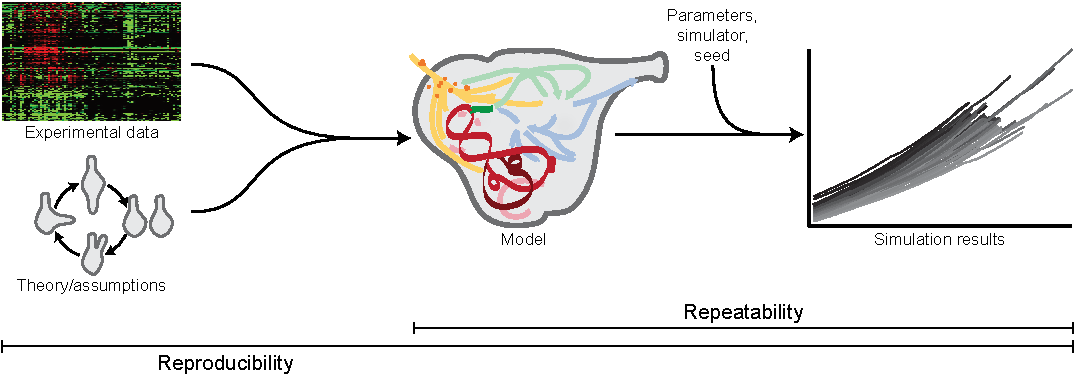
\includegraphics[width=\textwidth]{figure1/figure1}
% where an .eps filename suffix will be assumed under latex,
% and a .pdf suffix will be assumed for pdflatex; or what has been declared
% via \DeclareGraphicsExtensions.
\caption{Three requirements for reproducible systems biology modeling. (1) The provenance of every data source and assumption should be recorded so that models can be regenerated, including every species, reaction, and rate law.
(2) Every simulation parameter value should be recorded so that numerical simulation results can be regenerated. (3) Multiple simulation software tools should generate statistically identical numerical results. Reproducibility is a stricter standard than repeatability. Models are considered repeatable, but not reproducible, if they satisfy just the second and third criteria.}
\label{fig_repro_diagram}
\end{figure*}

These standards and modeling software tools help researchers repeat most systems biology simulation experiments and reuse, modify, expand, and combine most systems biology models. However, these standards and software provide limited support for regenerating models  because they do not record all design choices, such as experimental data sources and assumptions, that are used to build models,

Furthermore, researchers have begun to develop more complex models which cannot be represented by the existing standards or simulated by the existing standards-compliant software. For example, several aspects of the recent whole-cell (WC) model of \textit{Mycoplasma genitalium} \cite{Karr2012} cannot currently be represented by SBML \cite{Waltemath2016}. In particular, SBML cannot represent the multi-algorithmic nature of the model. In addition, no SBML-compatible simulation software program supports all of the SBML packages needed to simulate WC models, including the Arrays \cite{watanabe2016efficient}, Distributions \cite{Moodie2015}, Flux Balance Constraints \cite{olivier2015fbc}, Hierarchical Model Composition \cite{smith2015sbml}, and Multistate and Multicomponent Species \cite{SBMLMulti} packages.

Here, we present a path toward fully reproducible systems biology modeling, including WC modeling. First, we propose several requirements for reproducible modeling. Second, we outline several gaps in the existing standards and software for reproducible modeling and describe several new standards and software tools that are needed to achieve reproducible modeling. Third, we describe several methods for verifying repeatability. Achieving this vision will require significant research on standards and software development.

\section{The Requirements for Reproducible Modeling}

There are three requirements for fully reproducible systems biology modeling (Fig.~\ref{fig_repro_diagram}). (1) Researchers should be able to regenerate models, including every species and reaction from the literature. Consequently, researchers should record the provenance of every data source and assumption used to build models, as well as save a copy of each data source to guarantee future access to every source. (2) Researchers should be able to regenerate statistically identical simulation results. Consequently, researchers should record every parameter value, algorithm, and simulation software option used to simulate models. (3) Researchers should ensure that multiple simulation software tools generate statistically identical results. This is particularly helpful for identifying errors in complex simulation software programs. This requires standard model description formats that support all systems biology models, including WC models. This would enable researchers to use different software programs to generate the same results.

\section{Towards a Platform for Reproducible Modeling}

Currently, each individual modeler is responsible for reproducibly conducting their own research. This places a substantial burden on individual researchers to make every step of their research reproducible. To ease this burden, we recommend that the systems biology community develops several software tools, databases, and standards to enable researchers to conveniently conduct reproducible research.

(1) More comprehensive experimental databases should be developed to provide the data needed to build systems models.  For example, Karr et al. developed the WholeCellKB database \cite{karr2013wholecellkb} to organize the over 1,400 quantitative measurements used to build the \textit{M. genitalium} WC model. These databases should be machine-readable so that they can be automatically queried and used to build models. These databases should also use data models similar to that of systems biology models to clarify the connection between models and their underlying data. (2) New model design tools and Systems Biology Ontology (SBO) \cite{juty2013systems} terms are needed to record how models are built, including every design choice, assumption, and data source. Currently, researchers can use SBML annotations and SBO terms to record several common assumptions, such as the rapid equilibrium between free enzymes and enzyme-substrate complexes in Michaelis-Menten kinetics. However, many researchers do not utilize these annotations and the SBO does not represent all possible assumptions. Thus, researchers should develop model design tools which automatically record assumptions and data sources by adopting provenance tracking techniques \cite{callahan2006vistrails, hillman2012using, oinn2004taverna}. The SBO should also be expanded to represent more assumptions. (3) Where possible, researchers should use standard formats such as SBML and SED-ML rather than proprietary codes to describe models and simulation experiments. This should include annotation of the units of every parameter. (4) The existing standard model description formats should be expanded to represent all types of systems biology models, including WC models. For example, to describe WC models in a standard format, SBML could be expanded to support genomic sequence data and sequence-based reaction patterns or SBML could be linked with the Synthetic Biology Open Language (SBOL) \cite{galdzicki2014synthetic}, which is already capable of representing sequence data. (5) The existing standards-compliant simulation software programs should be expanded to support a wider variety of models. In particular, simulation software programs should be expanded to support the Arrays, Distributions, Flux Balance Constraints, Hierarchical Model Composition, and Multistate and Multicomponent Species SBML packages. Several simulation software programs, including BioUML \cite{Kolpakov2006} and iBioSim \cite{Stevens2013}, have already begun to support these packages. Unfortunately, most simulation software developers have insufficient funding to implement every package. (6) Modeling workflows should be expanded to systematically verify the statistical repeatability of simulation results. (7) New model verification tools should be developed to automatically identify errors in models. We developed a suite of tests to systematically error-check our \textit{M. genitalium} WC model\footnote{https://github.com/CovertLab/WholeCell/tree/master/src\_test}. These tests checked for simple problems such as undefined species, reaction mass and charge imbalance, and inconsistent reaction rates among submodels. Nevertheless, we found this test suite invaluable for debugging our model. These tests should be generalized and new software tools should be developed to help researchers systematically evaluate such tests. (8) Every model, simulation experiment, simulation result, and simulation software program should be reusable, extensible, documented, and published open-source \cite{easterbrook2014open}. (9) Journals should require and help authors permanently archive every reported data source and model.

\subsection{Special Considerations for Stochastic Simulation}
Stochastic simulations typically use pseudo-random number generators (PRNGs) which deterministically produce the same numbers when seeded with the same initial state. Therefore, we recommend that stochastic simulation software developers provide ways to set and record PRNG seeds so that modelers can repeat stochastic simulation results. This would enable researchers to repeat not only statistical distributions, but exact trajectories, which is invaluable for identifying and debugging errors in complex models and simulation algorithms.

Furthermore, different implementations of the same PRNG often differ in subtle ways. For example, the seed methods of the Boost C++ Library \cite{schaling2011boost} and Python Standard Library implementations of the Mersenne-Twister algorithm differentially initialize the PRNGs' internal states. Thus, we recommend the creation of standard PRNGs, including documentation of their algorithms, parameterizations, and initial states, and a test suite to help software developers verify their implementations.
 
\subsection{Special Considerations for Multi-algorithm WC Models}
Multi-algorithm WC models strive to represent every gene and cell function by combining multiple submodels of individual cellular pathways, each represented using different mathematics and each trained using different experimental data \cite{Karr2015, macklin2014future, carrera2015build}. For example, the \textit{M. genitalium} WC was composed of 28 submodels, including an FBA submodel which describes its metabolism, stochastic submodels which describes its transcription and translation, and an ODE submodel which describes its division. This multi-algorithm methodology is motivated by the desire to model biological systems as completely as possible, given our current knowledge, by simultaneously using fine-grained representations and coarse-grained representations to represent well- and poorly-characterized pathways, respectively.

Multi-algorithm modeling is a new methodology which still lacks a rigorous theoretical foundation. Consequently, significant work is needed to develop tools for building, simulating, and reproducing WC models. (1) The Hierarchical Model Composition SBML package should be extended to use the KiSAO ontology \cite{courtot2011controlled} to represent each submodel's simulation algorithm. (2) Researchers should determine how to concurrently integrate submodels that share state. Researchers are currently exploring several potential methods to concurrently integrate submodels, including shared memory and parallel discrete event simulation \cite{Goldberg2016}. (3) Researchers should develop a high-performance, reusable multi-algorithm simulator. (4) Additional tools should be developed to help researchers build and analyze WC models. (5) These programs should be implemented as separate tools and integrated into a comprehensive WC modeling platform so that software developers can contribute to individual tools and so that modelers can easily use alternative components. We anticipate that this platform will enable more researchers to engage in WC modeling and accelerate the WC modeling field.

\subsection{Special Considerations for Parallel Simulation Software Programs}

Multi-threaded and distributed computing are two important methods for accelerating the simulation of computationally expensive models such as WC models. Parallel programs use multiple threads and/or cores to simultaneously execute different parts of a simulation. The order in which these threads and/or cores complete computations depends on the operating environment, and the order in which computations complete can affect subsequent computations and, in turn, simulation results. Other sources of non-determinism in parallel computing include memory layout, delays caused by devices and processes, and user input. Thus, parallel programs can generate non-deterministic simulation results due to variable operating environments.

For example, if two WC submodels which are executed in parallel attempt to bind proteins to the same site on the chromosome, the submodel which completes its computations first will bind the protein to the chromosome. However, when the simulation is re-run under a different load on the computer, the other submodel may complete its computations first, resulting in the binding of a different protein the site. This small difference can lead to further differences between later time steps, resulting in different simulation results solely due to different operating environments.

Consequently, special care must be taken to create deterministic parallel simulation programs. Therefore, we briefly examine methods from computer science which have been developed to create deterministic parallel programs.

\begin{figure*}
  \centering
  \begin{subfigure}[b]{0.5\textwidth}
    \centering
    \[
    \begin{array}{c c c}
       & \textrm{Reaction} & \textrm{Rate} \\
      \left( 1 \right) & \varnothing \to x & \frac{1}{2} + V_m \frac{x^n}{K_m + x^n} \\ \\
      \left( 2 \right) & x \to \varnothing & \frac{k}{x} \\ \\
    \end{array}
    \]
    Where
    \[
      x = 24\,\SI{}{\micro\Molar} ~ \textrm{at} ~ t = 0\,s,
    \]
    \[
      n = 4,
    \]
    \[
      V_m = 4\,s^{-1},
    \]
    \[
      K_m = 10^6\,\SI{}{\micro\Molar}\text{, and}
    \]
    \[
      k = 0.125\,\SI{}{\micro\Molar}\,s^{-1}.
    \]
    \vspace{1em}
  \end{subfigure}%
  \begin{subfigure}[b]{0.5\textwidth}
    \centering
    % This file was created by matplotlib2tikz v0.5.4.
% The lastest updates can be retrieved from
% 
% https://github.com/nschloe/matplotlib2tikz
% 
% where you can also submit bug reports and leavecomments.
% 
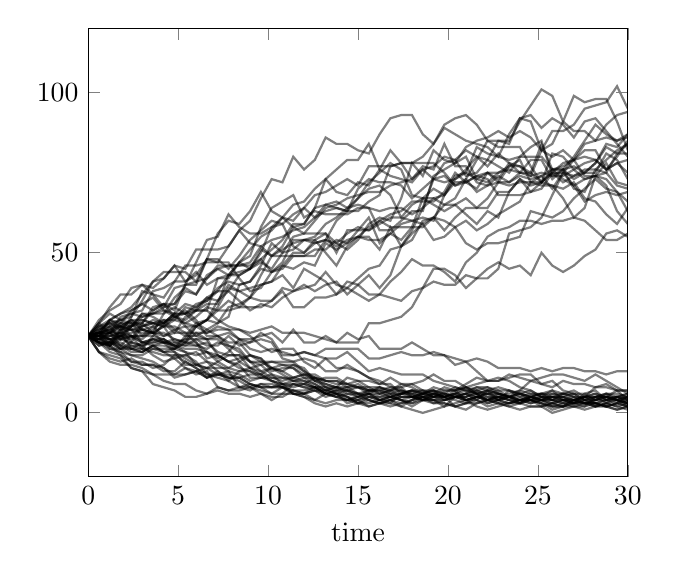
\begin{tikzpicture}

\begin{axis}[
xlabel={time},
xmin=0, xmax=30,
ymin=-20, ymax=120,
axis on top
]
\addplot [thick, black, opacity=0.5]
table {%
0 23.88
0.6 23.88
1.2 20.88
1.8 18.88
2.4 17.88
3 16.88
3.6 15.88
4.2 13.88
4.8 10.88
5.4 11.88
6 12.88
6.6 10.88
7.2 11.88
7.8 10.88
8.4 9.88
9 7.88
9.6 8.88
10.2 7.88
10.8 7.88
11.4 5.88
12 4.88
12.6 3.88
13.2 5.88
13.8 4.88
14.4 3.88
15 4.88
15.6 5.88
16.2 3.88
16.8 4.88
17.4 3.88
18 4.88
18.6 3.88
19.2 4.88
19.8 6.88
20.4 6.88
21 7.88
21.6 5.88
22.2 3.88
22.8 4.88
23.4 5.88
24 6.88
24.6 9.88
25.2 8.88
25.8 9.88
26.4 6.88
27 5.88
27.6 5.88
28.2 3.88
28.8 5.88
29.4 4.88
30 3.88
};
\addplot [thick, black, opacity=0.5]
table {%
0 23.88
0.6 23.88
1.2 28.88
1.8 30.88
2.4 31.88
3 33.88
3.6 31.88
4.2 33.88
4.8 33.88
5.4 39.88
6 46.88
6.6 53.88
7.2 54.88
7.8 61.88
8.4 57.88
9 55.88
9.6 55.88
10.2 57.88
10.8 60.88
11.4 57.88
12 58.88
12.6 63.88
13.2 64.88
13.8 65.88
14.4 63.88
15 64.88
15.6 63.88
16.2 56.88
16.8 56.88
17.4 59.88
18 62.88
18.6 62.88
19.2 73.88
19.8 75.88
20.4 77.88
21 82.88
21.6 84.88
22.2 85.88
22.8 87.88
23.4 85.88
24 87.88
24.6 85.88
25.2 81.88
25.8 87.88
26.4 87.88
27 89.88
27.6 94.88
28.2 95.88
28.8 96.88
29.4 101.88
30 94.88
};
\addplot [thick, black, opacity=0.5]
table {%
0 23.88
0.6 24.88
1.2 24.88
1.8 25.88
2.4 26.88
3 27.88
3.6 24.88
4.2 24.88
4.8 22.88
5.4 21.88
6 20.88
6.6 19.88
7.2 21.88
7.8 20.88
8.4 19.88
9 15.88
9.6 15.88
10.2 13.88
10.8 12.88
11.4 10.88
12 11.88
12.6 9.88
13.2 10.88
13.8 10.88
14.4 8.88
15 7.88
15.6 6.88
16.2 6.88
16.8 5.88
17.4 3.88
18 1.88
18.6 3.88
19.2 3.88
19.8 2.88
20.4 1.88
21 0.879999999999999
21.6 2.88
22.2 3.88
22.8 5.88
23.4 4.88
24 3.88
24.6 4.88
25.2 3.88
25.8 2.88
26.4 3.88
27 2.88
27.6 2.88
28.2 1.88
28.8 2.88
29.4 1.88
30 0.879999999999999
};
\addplot [thick, black, opacity=0.5]
table {%
0 23.88
0.6 23.88
1.2 24.88
1.8 29.88
2.4 30.88
3 31.88
3.6 37.88
4.2 38.88
4.8 40.88
5.4 45.88
6 45.88
6.6 46.88
7.2 46.88
7.8 46.88
8.4 41.88
9 37.88
9.6 38.88
10.2 43.88
10.8 46.88
11.4 53.88
12 53.88
12.6 54.88
13.2 58.88
13.8 60.88
14.4 63.88
15 66.88
15.6 71.88
16.2 74.88
16.8 77.88
17.4 75.88
18 67.88
18.6 66.88
19.2 64.88
19.8 62.88
20.4 64.88
21 66.88
21.6 63.88
22.2 66.88
22.8 71.88
23.4 76.88
24 76.88
24.6 74.88
25.2 71.88
25.8 80.88
26.4 79.88
27 75.88
27.6 72.88
28.2 73.88
28.8 70.88
29.4 62.88
30 58.88
};
\addplot [thick, black, opacity=0.5]
table {%
0 23.88
0.6 23.88
1.2 26.88
1.8 26.88
2.4 23.88
3 19.88
3.6 18.88
4.2 17.88
4.8 17.88
5.4 15.88
6 13.88
6.6 11.88
7.2 11.88
7.8 10.88
8.4 10.88
9 11.88
9.6 11.88
10.2 13.88
10.8 11.88
11.4 9.88
12 9.88
12.6 8.88
13.2 6.88
13.8 5.88
14.4 4.88
15 2.88
15.6 3.88
16.2 2.88
16.8 3.88
17.4 4.88
18 4.88
18.6 3.88
19.2 4.88
19.8 5.88
20.4 7.88
21 6.88
21.6 5.88
22.2 3.88
22.8 2.88
23.4 1.88
24 2.88
24.6 4.88
25.2 3.88
25.8 4.88
26.4 5.88
27 6.88
27.6 4.88
28.2 4.88
28.8 4.88
29.4 3.88
30 2.88
};
\addplot [thick, black, opacity=0.5]
table {%
0 23.88
0.6 25.88
1.2 27.88
1.8 26.88
2.4 28.88
3 26.88
3.6 27.88
4.2 26.88
4.8 29.88
5.4 28.88
6 31.88
6.6 31.88
7.2 41.88
7.8 41.88
8.4 46.88
9 50.88
9.6 54.88
10.2 56.88
10.8 60.88
11.4 59.88
12 63.88
12.6 60.88
13.2 62.88
13.8 63.88
14.4 62.88
15 69.88
15.6 72.88
16.2 71.88
16.8 71.88
17.4 70.88
18 66.88
18.6 69.88
19.2 72.88
19.8 77.88
20.4 78.88
21 73.88
21.6 74.88
22.2 78.88
22.8 76.88
23.4 74.88
24 79.88
24.6 82.88
25.2 84.88
25.8 73.88
26.4 73.88
27 75.88
27.6 77.88
28.2 78.88
28.8 75.88
29.4 77.88
30 74.88
};
\addplot [thick, black, opacity=0.5]
table {%
0 23.88
0.6 24.88
1.2 24.88
1.8 26.88
2.4 25.88
3 21.88
3.6 22.88
4.2 21.88
4.8 18.88
5.4 16.88
6 14.88
6.6 15.88
7.2 14.88
7.8 12.88
8.4 7.88
9 8.88
9.6 7.88
10.2 7.88
10.8 7.88
11.4 5.88
12 5.88
12.6 6.88
13.2 6.88
13.8 5.88
14.4 2.88
15 3.88
15.6 1.88
16.2 2.88
16.8 3.88
17.4 2.88
18 3.88
18.6 4.88
19.2 2.88
19.8 3.88
20.4 4.88
21 3.88
21.6 3.88
22.2 1.88
22.8 2.88
23.4 1.88
24 0.879999999999999
24.6 1.88
25.2 1.88
25.8 2.88
26.4 3.88
27 3.88
27.6 2.88
28.2 3.88
28.8 4.88
29.4 3.88
30 2.88
};
\addplot [thick, black, opacity=0.5]
table {%
0 23.88
0.6 21.88
1.2 21.88
1.8 19.88
2.4 20.88
3 19.88
3.6 19.88
4.2 18.88
4.8 19.88
5.4 18.88
6 17.88
6.6 18.88
7.2 15.88
7.8 13.88
8.4 12.88
9 13.88
9.6 12.88
10.2 10.88
10.8 9.88
11.4 10.88
12 9.88
12.6 7.88
13.2 5.88
13.8 4.88
14.4 5.88
15 5.88
15.6 5.88
16.2 4.88
16.8 4.88
17.4 3.88
18 2.88
18.6 3.88
19.2 3.88
19.8 1.88
20.4 4.88
21 4.88
21.6 6.88
22.2 4.88
22.8 4.88
23.4 4.88
24 4.88
24.6 3.88
25.2 1.88
25.8 -0.120000000000001
26.4 0.879999999999999
27 1.88
27.6 2.88
28.2 2.88
28.8 1.88
29.4 0.879999999999999
30 1.88
};
\addplot [thick, black, opacity=0.5]
table {%
0 23.88
0.6 27.88
1.2 32.88
1.8 36.88
2.4 36.88
3 39.88
3.6 38.88
4.2 41.88
4.8 45.88
5.4 40.88
6 42.88
6.6 47.88
7.2 55.88
7.8 59.88
8.4 58.88
9 62.88
9.6 68.88
10.2 62.88
10.8 60.88
11.4 64.88
12 65.88
12.6 69.88
13.2 72.88
13.8 68.88
14.4 67.88
15 71.88
15.6 70.88
16.2 75.88
16.8 73.88
17.4 72.88
18 71.88
18.6 75.88
19.2 72.88
19.8 71.88
20.4 72.88
21 74.88
21.6 72.88
22.2 71.88
22.8 74.88
23.4 76.88
24 78.88
24.6 71.88
25.2 73.88
25.8 75.88
26.4 76.88
27 78.88
27.6 73.88
28.2 73.88
28.8 72.88
29.4 68.88
30 62.88
};
\addplot [thick, black, opacity=0.5]
table {%
0 23.88
0.6 23.88
1.2 23.88
1.8 24.88
2.4 29.88
3 34.88
3.6 40.88
4.2 43.88
4.8 43.88
5.4 43.88
6 40.88
6.6 47.88
7.2 47.88
7.8 44.88
8.4 48.88
9 53.88
9.6 56.88
10.2 59.88
10.8 58.88
11.4 51.88
12 49.88
12.6 52.88
13.2 53.88
13.8 51.88
14.4 53.88
15 54.88
15.6 53.88
16.2 53.88
16.8 55.88
17.4 53.88
18 57.88
18.6 66.88
19.2 69.88
19.8 67.88
20.4 72.88
21 75.88
21.6 79.88
22.2 76.88
22.8 80.88
23.4 77.88
24 74.88
24.6 73.88
25.2 74.88
25.8 73.88
26.4 75.88
27 69.88
27.6 68.88
28.2 75.88
28.8 78.88
29.4 81.88
30 83.88
};
\addplot [thick, black, opacity=0.5]
table {%
0 23.88
0.6 21.88
1.2 20.88
1.8 22.88
2.4 23.88
3 22.88
3.6 25.88
4.2 28.88
4.8 28.88
5.4 32.88
6 31.88
6.6 35.88
7.2 34.88
7.8 37.88
8.4 42.88
9 44.88
9.6 49.88
10.2 57.88
10.8 58.88
11.4 61.88
12 63.88
12.6 67.88
13.2 68.88
13.8 70.88
14.4 72.88
15 70.88
15.6 76.88
16.2 76.88
16.8 76.88
17.4 77.88
18 72.88
18.6 75.88
19.2 76.88
19.8 79.88
20.4 78.88
21 81.88
21.6 79.88
22.2 78.88
22.8 84.88
23.4 84.88
24 90.88
24.6 95.88
25.2 100.88
25.8 98.88
26.4 90.88
27 98.88
27.6 96.88
28.2 97.88
28.8 97.88
29.4 90.88
30 81.88
};
\addplot [thick, black, opacity=0.5]
table {%
0 23.88
0.6 24.88
1.2 25.88
1.8 26.88
2.4 26.88
3 30.88
3.6 30.88
4.2 32.88
4.8 33.88
5.4 37.88
6 36.88
6.6 41.88
7.2 44.88
7.8 45.88
8.4 45.88
9 45.88
9.6 47.88
10.2 43.88
10.8 44.88
11.4 48.88
12 48.88
12.6 48.88
13.2 53.88
13.8 52.88
14.4 55.88
15 57.88
15.6 56.88
16.2 59.88
16.8 57.88
17.4 57.88
18 57.88
18.6 57.88
19.2 60.88
19.8 59.88
20.4 57.88
21 52.88
21.6 50.88
22.2 52.88
22.8 52.88
23.4 53.88
24 54.88
24.6 62.88
25.2 61.88
25.8 60.88
26.4 62.88
27 66.88
27.6 69.88
28.2 72.88
28.8 69.88
29.4 68.88
30 65.88
};
\addplot [thick, black, opacity=0.5]
table {%
0 23.88
0.6 25.88
1.2 27.88
1.8 28.88
2.4 30.88
3 29.88
3.6 30.88
4.2 31.88
4.8 29.88
5.4 30.88
6 32.88
6.6 35.88
7.2 37.88
7.8 42.88
8.4 46.88
9 48.88
9.6 57.88
10.2 63.88
10.8 65.88
11.4 67.88
12 60.88
12.6 62.88
13.2 61.88
13.8 61.88
14.4 61.88
15 63.88
15.6 63.88
16.2 62.88
16.8 63.88
17.4 63.88
18 61.88
18.6 63.88
19.2 66.88
19.8 64.88
20.4 64.88
21 61.88
21.6 58.88
22.2 62.88
22.8 60.88
23.4 68.88
24 72.88
24.6 68.88
25.2 69.88
25.8 74.88
26.4 77.88
27 78.88
27.6 81.88
28.2 81.88
28.8 75.88
29.4 79.88
30 84.88
};
\addplot [thick, black, opacity=0.5]
table {%
0 23.88
0.6 24.88
1.2 26.88
1.8 22.88
2.4 26.88
3 28.88
3.6 27.88
4.2 28.88
4.8 25.88
5.4 26.88
6 23.88
6.6 22.88
7.2 23.88
7.8 24.88
8.4 22.88
9 21.88
9.6 22.88
10.2 21.88
10.8 16.88
11.4 15.88
12 16.88
12.6 15.88
13.2 12.88
13.8 12.88
14.4 14.88
15 12.88
15.6 10.88
16.2 9.88
16.8 7.88
17.4 7.88
18 4.88
18.6 5.88
19.2 6.88
19.8 4.88
20.4 5.88
21 5.88
21.6 7.88
22.2 6.88
22.8 3.88
23.4 2.88
24 2.88
24.6 1.88
25.2 1.88
25.8 2.88
26.4 1.88
27 3.88
27.6 4.88
28.2 4.88
28.8 2.88
29.4 3.88
30 2.88
};
\addplot [thick, black, opacity=0.5]
table {%
0 23.88
0.6 20.88
1.2 21.88
1.8 20.88
2.4 18.88
3 18.88
3.6 20.88
4.2 20.88
4.8 19.88
5.4 23.88
6 23.88
6.6 25.88
7.2 27.88
7.8 32.88
8.4 33.88
9 35.88
9.6 42.88
10.2 48.88
10.8 51.88
11.4 57.88
12 55.88
12.6 59.88
13.2 63.88
13.8 64.88
14.4 66.88
15 67.88
15.6 68.88
16.2 68.88
16.8 70.88
17.4 71.88
18 72.88
18.6 76.88
19.2 75.88
19.8 83.88
20.4 76.88
21 76.88
21.6 71.88
22.2 70.88
22.8 71.88
23.4 70.88
24 71.88
24.6 71.88
25.2 71.88
25.8 70.88
26.4 66.88
27 60.88
27.6 63.88
28.2 73.88
28.8 77.88
29.4 71.88
30 70.88
};
\addplot [thick, black, opacity=0.5]
table {%
0 23.88
0.6 18.88
1.2 15.88
1.8 14.88
2.4 14.88
3 13.88
3.6 11.88
4.2 11.88
4.8 11.88
5.4 13.88
6 11.88
6.6 12.88
7.2 7.88
7.8 6.88
8.4 6.88
9 7.88
9.6 5.88
10.2 3.88
10.8 5.88
11.4 8.88
12 7.88
12.6 6.88
13.2 5.88
13.8 6.88
14.4 4.88
15 2.88
15.6 4.88
16.2 3.88
16.8 3.88
17.4 1.88
18 0.879999999999999
18.6 -0.120000000000001
19.2 0.879999999999999
19.8 1.88
20.4 2.88
21 3.88
21.6 4.88
22.2 5.88
22.8 6.88
23.4 6.88
24 5.88
24.6 6.88
25.2 4.88
25.8 3.88
26.4 2.88
27 2.88
27.6 5.88
28.2 6.88
28.8 3.88
29.4 4.88
30 5.88
};
\addplot [thick, black, opacity=0.5]
table {%
0 23.88
0.6 24.88
1.2 23.88
1.8 24.88
2.4 23.88
3 23.88
3.6 26.88
4.2 27.88
4.8 30.88
5.4 33.88
6 32.88
6.6 34.88
7.2 38.88
7.8 40.88
8.4 39.88
9 40.88
9.6 44.88
10.2 43.88
10.8 45.88
11.4 49.88
12 49.88
12.6 53.88
13.2 55.88
13.8 49.88
14.4 56.88
15 56.88
15.6 56.88
16.2 58.88
16.8 60.88
17.4 60.88
18 59.88
18.6 58.88
19.2 60.88
19.8 64.88
20.4 66.88
21 72.88
21.6 78.88
22.2 84.88
22.8 82.88
23.4 82.88
24 82.88
24.6 76.88
25.2 71.88
25.8 75.88
26.4 72.88
27 70.88
27.6 65.88
28.2 67.88
28.8 68.88
29.4 67.88
30 68.88
};
\addplot [thick, black, opacity=0.5]
table {%
0 23.88
0.6 24.88
1.2 22.88
1.8 23.88
2.4 24.88
3 25.88
3.6 24.88
4.2 21.88
4.8 22.88
5.4 21.88
6 21.88
6.6 16.88
7.2 17.88
7.8 15.88
8.4 16.88
9 17.88
9.6 16.88
10.2 13.88
10.8 14.88
11.4 13.88
12 11.88
12.6 10.88
13.2 7.88
13.8 7.88
14.4 6.88
15 4.88
15.6 5.88
16.2 7.88
16.8 5.88
17.4 6.88
18 5.88
18.6 4.88
19.2 3.88
19.8 4.88
20.4 6.88
21 7.88
21.6 5.88
22.2 6.88
22.8 5.88
23.4 4.88
24 3.88
24.6 4.88
25.2 3.88
25.8 3.88
26.4 3.88
27 2.88
27.6 3.88
28.2 2.88
28.8 3.88
29.4 4.88
30 3.88
};
\addplot [thick, black, opacity=0.5]
table {%
0 23.88
0.6 21.88
1.2 19.88
1.8 19.88
2.4 21.88
3 26.88
3.6 27.88
4.2 26.88
4.8 21.88
5.4 22.88
6 22.88
6.6 20.88
7.2 20.88
7.8 23.88
8.4 20.88
9 21.88
9.6 24.88
10.2 22.88
10.8 17.88
11.4 17.88
12 18.88
12.6 17.88
13.2 16.88
13.8 16.88
14.4 18.88
15 15.88
15.6 12.88
16.2 13.88
16.8 12.88
17.4 11.88
18 11.88
18.6 11.88
19.2 9.88
19.8 8.88
20.4 7.88
21 6.88
21.6 7.88
22.2 7.88
22.8 5.88
23.4 4.88
24 5.88
24.6 3.88
25.2 4.88
25.8 3.88
26.4 4.88
27 2.88
27.6 3.88
28.2 1.88
28.8 2.88
29.4 4.88
30 2.88
};
\addplot [thick, black, opacity=0.5]
table {%
0 23.88
0.6 23.88
1.2 22.88
1.8 23.88
2.4 22.88
3 27.88
3.6 31.88
4.2 33.88
4.8 31.88
5.4 39.88
6 39.88
6.6 47.88
7.2 46.88
7.8 51.88
8.4 56.88
9 59.88
9.6 66.88
10.2 72.88
10.8 71.88
11.4 79.88
12 75.88
12.6 78.88
13.2 85.88
13.8 83.88
14.4 83.88
15 81.88
15.6 80.88
16.2 86.88
16.8 91.88
17.4 92.88
18 92.88
18.6 86.88
19.2 83.88
19.8 89.88
20.4 91.88
21 92.88
21.6 89.88
22.2 84.88
22.8 84.88
23.4 83.88
24 91.88
24.6 90.88
25.2 81.88
25.8 83.88
26.4 90.88
27 87.88
27.6 87.88
28.2 84.88
28.8 85.88
29.4 84.88
30 85.88
};
\addplot [thick, black, opacity=0.5]
table {%
0 23.88
0.6 24.88
1.2 28.88
1.8 30.88
2.4 32.88
3 36.88
3.6 40.88
4.2 41.88
4.8 45.88
5.4 44.88
6 50.88
6.6 50.88
7.2 50.88
7.8 51.88
8.4 56.88
9 52.88
9.6 51.88
10.2 48.88
10.8 50.88
11.4 52.88
12 53.88
12.6 52.88
13.2 53.88
13.8 59.88
14.4 62.88
15 62.88
15.6 65.88
16.2 67.88
16.8 76.88
17.4 77.88
18 77.88
18.6 79.88
19.2 83.88
19.8 88.88
20.4 86.88
21 84.88
21.6 83.88
22.2 82.88
22.8 79.88
23.4 86.88
24 91.88
24.6 92.88
25.2 88.88
25.8 91.88
26.4 89.88
27 85.88
27.6 90.88
28.2 91.88
28.8 87.88
29.4 83.88
30 79.88
};
\addplot [thick, black, opacity=0.5]
table {%
0 23.88
0.6 24.88
1.2 20.88
1.8 24.88
2.4 25.88
3 24.88
3.6 24.88
4.2 26.88
4.8 28.88
5.4 27.88
6 26.88
6.6 24.88
7.2 26.88
7.8 25.88
8.4 25.88
9 23.88
9.6 20.88
10.2 18.88
10.8 19.88
11.4 19.88
12 15.88
12.6 13.88
13.2 16.88
13.8 13.88
14.4 13.88
15 12.88
15.6 10.88
16.2 8.88
16.8 8.88
17.4 5.88
18 6.88
18.6 5.88
19.2 6.88
19.8 5.88
20.4 4.88
21 5.88
21.6 6.88
22.2 7.88
22.8 6.88
23.4 4.88
24 3.88
24.6 3.88
25.2 4.88
25.8 4.88
26.4 4.88
27 3.88
27.6 2.88
28.2 1.88
28.8 1.88
29.4 2.88
30 1.88
};
\addplot [thick, black, opacity=0.5]
table {%
0 23.88
0.6 21.88
1.2 20.88
1.8 23.88
2.4 27.88
3 23.88
3.6 24.88
4.2 26.88
4.8 26.88
5.4 24.88
6 24.88
6.6 22.88
7.2 17.88
7.8 15.88
8.4 13.88
9 12.88
9.6 10.88
10.2 9.88
10.8 7.88
11.4 6.88
12 6.88
12.6 7.88
13.2 6.88
13.8 7.88
14.4 5.88
15 4.88
15.6 6.88
16.2 6.88
16.8 7.88
17.4 6.88
18 5.88
18.6 3.88
19.2 5.88
19.8 7.88
20.4 6.88
21 3.88
21.6 4.88
22.2 4.88
22.8 3.88
23.4 4.88
24 3.88
24.6 4.88
25.2 3.88
25.8 1.88
26.4 1.88
27 2.88
27.6 2.88
28.2 3.88
28.8 3.88
29.4 2.88
30 3.88
};
\addplot [thick, black, opacity=0.5]
table {%
0 23.88
0.6 22.88
1.2 22.88
1.8 20.88
2.4 23.88
3 21.88
3.6 22.88
4.2 22.88
4.8 19.88
5.4 21.88
6 24.88
6.6 24.88
7.2 25.88
7.8 25.88
8.4 22.88
9 19.88
9.6 18.88
10.2 19.88
10.8 18.88
11.4 17.88
12 18.88
12.6 17.88
13.2 19.88
13.8 19.88
14.4 19.88
15 19.88
15.6 16.88
16.2 16.88
16.8 17.88
17.4 18.88
18 17.88
18.6 17.88
19.2 18.88
19.8 17.88
20.4 16.88
21 15.88
21.6 12.88
22.2 9.88
22.8 9.88
23.4 11.88
24 10.88
24.6 9.88
25.2 10.88
25.8 11.88
26.4 11.88
27 10.88
27.6 9.88
28.2 11.88
28.8 9.88
29.4 7.88
30 5.88
};
\addplot [thick, black, opacity=0.5]
table {%
0 23.88
0.6 21.88
1.2 21.88
1.8 25.88
2.4 25.88
3 26.88
3.6 28.88
4.2 27.88
4.8 24.88
5.4 29.88
6 31.88
6.6 33.88
7.2 33.88
7.8 42.88
8.4 43.88
9 44.88
9.6 47.88
10.2 50.88
10.8 53.88
11.4 58.88
12 58.88
12.6 63.88
13.2 72.88
13.8 75.88
14.4 78.88
15 78.88
15.6 83.88
16.2 75.88
16.8 81.88
17.4 77.88
18 77.88
18.6 77.88
19.2 77.88
19.8 74.88
20.4 70.88
21 72.88
21.6 68.88
22.2 70.88
22.8 73.88
23.4 71.88
24 73.88
24.6 72.88
25.2 73.88
25.8 69.88
26.4 74.88
27 78.88
27.6 79.88
28.2 78.88
28.8 75.88
29.4 77.88
30 78.88
};
\addplot [thick, black, opacity=0.5]
table {%
0 23.88
0.6 27.88
1.2 24.88
1.8 27.88
2.4 31.88
3 33.88
3.6 35.88
4.2 31.88
4.8 30.88
5.4 30.88
6 27.88
6.6 28.88
7.2 27.88
7.8 29.88
8.4 39.88
9 40.88
9.6 45.88
10.2 52.88
10.8 49.88
11.4 50.88
12 53.88
12.6 53.88
13.2 49.88
13.8 45.88
14.4 51.88
15 54.88
15.6 54.88
16.2 50.88
16.8 57.88
17.4 51.88
18 55.88
18.6 58.88
19.2 53.88
19.8 54.88
20.4 57.88
21 59.88
21.6 56.88
22.2 58.88
22.8 61.88
23.4 63.88
24 65.88
24.6 71.88
25.2 70.88
25.8 70.88
26.4 69.88
27 71.88
27.6 66.88
28.2 65.88
28.8 61.88
29.4 58.88
30 63.88
};
\addplot [thick, black, opacity=0.5]
table {%
0 23.88
0.6 18.88
1.2 16.88
1.8 15.88
2.4 16.88
3 14.88
3.6 14.88
4.2 12.88
4.8 12.88
5.4 15.88
6 13.88
6.6 10.88
7.2 12.88
7.8 9.88
8.4 12.88
9 12.88
9.6 11.88
10.2 9.88
10.8 8.88
11.4 9.88
12 10.88
12.6 10.88
13.2 8.88
13.8 7.88
14.4 10.88
15 9.88
15.6 7.88
16.2 7.88
16.8 6.88
17.4 4.88
18 4.88
18.6 5.88
19.2 4.88
19.8 5.88
20.4 4.88
21 4.88
21.6 5.88
22.2 6.88
22.8 5.88
23.4 4.88
24 2.88
24.6 4.88
25.2 3.88
25.8 2.88
26.4 1.88
27 2.88
27.6 4.88
28.2 5.88
28.8 3.88
29.4 4.88
30 5.88
};
\addplot [thick, black, opacity=0.5]
table {%
0 23.88
0.6 22.88
1.2 24.88
1.8 24.88
2.4 19.88
3 19.88
3.6 23.88
4.2 27.88
4.8 29.88
5.4 27.88
6 29.88
6.6 32.88
7.2 31.88
7.8 31.88
8.4 32.88
9 32.88
9.6 32.88
10.2 34.88
10.8 38.88
11.4 37.88
12 39.88
12.6 37.88
13.2 39.88
13.8 40.88
14.4 36.88
15 39.88
15.6 42.88
16.2 38.88
16.8 42.88
17.4 51.88
18 56.88
18.6 63.88
19.2 72.88
19.8 73.88
20.4 70.88
21 71.88
21.6 73.88
22.2 72.88
22.8 67.88
23.4 67.88
24 67.88
24.6 68.88
25.2 71.88
25.8 74.88
26.4 74.88
27 70.88
27.6 72.88
28.2 73.88
28.8 74.88
29.4 70.88
30 69.88
};
\addplot [thick, black, opacity=0.5]
table {%
0 23.88
0.6 26.88
1.2 27.88
1.8 25.88
2.4 28.88
3 28.88
3.6 27.88
4.2 27.88
4.8 30.88
5.4 30.88
6 33.88
6.6 34.88
7.2 37.88
7.8 37.88
8.4 34.88
9 31.88
9.6 33.88
10.2 32.88
10.8 35.88
11.4 37.88
12 38.88
12.6 39.88
13.2 43.88
13.8 39.88
14.4 38.88
15 36.88
15.6 34.88
16.2 36.88
16.8 40.88
17.4 43.88
18 47.88
18.6 45.88
19.2 45.88
19.8 43.88
20.4 40.88
21 46.88
21.6 49.88
22.2 54.88
22.8 56.88
23.4 57.88
24 59.88
24.6 59.88
25.2 58.88
25.8 59.88
26.4 59.88
27 60.88
27.6 59.88
28.2 56.88
28.8 53.88
29.4 53.88
30 55.88
};
\addplot [thick, black, opacity=0.5]
table {%
0 23.88
0.6 21.88
1.2 20.88
1.8 17.88
2.4 15.88
3 15.88
3.6 13.88
4.2 14.88
4.8 17.88
5.4 17.88
6 15.88
6.6 11.88
7.2 10.88
7.8 9.88
8.4 7.88
9 6.88
9.6 8.88
10.2 8.88
10.8 7.88
11.4 8.88
12 7.88
12.6 7.88
13.2 5.88
13.8 4.88
14.4 3.88
15 4.88
15.6 3.88
16.2 2.88
16.8 2.88
17.4 5.88
18 6.88
18.6 5.88
19.2 4.88
19.8 3.88
20.4 4.88
21 3.88
21.6 1.88
22.2 0.879999999999999
22.8 1.88
23.4 2.88
24 3.88
24.6 2.88
25.2 3.88
25.8 4.88
26.4 3.88
27 3.88
27.6 4.88
28.2 7.88
28.8 7.88
29.4 6.88
30 6.88
};
\addplot [thick, black, opacity=0.5]
table {%
0 23.88
0.6 24.88
1.2 21.88
1.8 21.88
2.4 19.88
3 21.88
3.6 20.88
4.2 21.88
4.8 20.88
5.4 18.88
6 14.88
6.6 13.88
7.2 13.88
7.8 13.88
8.4 15.88
9 13.88
9.6 14.88
10.2 11.88
10.8 10.88
11.4 9.88
12 8.88
12.6 7.88
13.2 5.88
13.8 5.88
14.4 3.88
15 2.88
15.6 1.88
16.2 2.88
16.8 1.88
17.4 2.88
18 3.88
18.6 5.88
19.2 7.88
19.8 6.88
20.4 6.88
21 8.88
21.6 10.88
22.2 9.88
22.8 10.88
23.4 9.88
24 7.88
24.6 6.88
25.2 4.88
25.8 6.88
26.4 3.88
27 4.88
27.6 3.88
28.2 4.88
28.8 4.88
29.4 3.88
30 2.88
};
\addplot [thick, black, opacity=0.5]
table {%
0 23.88
0.6 24.88
1.2 28.88
1.8 27.88
2.4 26.88
3 30.88
3.6 29.88
4.2 27.88
4.8 30.88
5.4 26.88
6 26.88
6.6 28.88
7.2 31.88
7.8 34.88
8.4 32.88
9 35.88
9.6 34.88
10.2 34.88
10.8 37.88
11.4 32.88
12 32.88
12.6 35.88
13.2 35.88
13.8 36.88
14.4 40.88
15 39.88
15.6 36.88
16.2 36.88
16.8 35.88
17.4 34.88
18 37.88
18.6 38.88
19.2 44.88
19.8 44.88
20.4 42.88
21 38.88
21.6 41.88
22.2 44.88
22.8 46.88
23.4 44.88
24 45.88
24.6 42.88
25.2 49.88
25.8 45.88
26.4 43.88
27 45.88
27.6 48.88
28.2 50.88
28.8 55.88
29.4 56.88
30 54.88
};
\addplot [thick, black, opacity=0.5]
table {%
0 23.88
0.6 22.88
1.2 21.88
1.8 23.88
2.4 26.88
3 29.88
3.6 30.88
4.2 30.88
4.8 32.88
5.4 30.88
6 31.88
6.6 31.88
7.2 28.88
7.8 26.88
8.4 25.88
9 24.88
9.6 25.88
10.2 26.88
10.8 24.88
11.4 24.88
12 24.88
12.6 23.88
13.2 22.88
13.8 21.88
14.4 24.88
15 22.88
15.6 23.88
16.2 19.88
16.8 19.88
17.4 19.88
18 21.88
18.6 19.88
19.2 17.88
19.8 17.88
20.4 14.88
21 15.88
21.6 16.88
22.2 15.88
22.8 13.88
23.4 13.88
24 13.88
24.6 12.88
25.2 13.88
25.8 12.88
26.4 13.88
27 13.88
27.6 12.88
28.2 12.88
28.8 11.88
29.4 12.88
30 12.88
};
\addplot [thick, black, opacity=0.5]
table {%
0 23.88
0.6 24.88
1.2 25.88
1.8 23.88
2.4 23.88
3 21.88
3.6 21.88
4.2 21.88
4.8 20.88
5.4 20.88
6 22.88
6.6 22.88
7.2 22.88
7.8 19.88
8.4 15.88
9 17.88
9.6 15.88
10.2 15.88
10.8 15.88
11.4 15.88
12 12.88
12.6 10.88
13.2 9.88
13.8 9.88
14.4 8.88
15 9.88
15.6 9.88
16.2 8.88
16.8 10.88
17.4 8.88
18 8.88
18.6 9.88
19.2 11.88
19.8 9.88
20.4 9.88
21 7.88
21.6 8.88
22.2 9.88
22.8 9.88
23.4 10.88
24 11.88
24.6 11.88
25.2 8.88
25.8 7.88
26.4 9.88
27 8.88
27.6 8.88
28.2 7.88
28.8 8.88
29.4 6.88
30 3.88
};
\addplot [thick, black, opacity=0.5]
table {%
0 23.88
0.6 22.88
1.2 24.88
1.8 20.88
2.4 19.88
3 18.88
3.6 20.88
4.2 18.88
4.8 16.88
5.4 17.88
6 18.88
6.6 15.88
7.2 12.88
7.8 10.88
8.4 10.88
9 8.88
9.6 7.88
10.2 5.88
10.8 7.88
11.4 6.88
12 5.88
12.6 6.88
13.2 4.88
13.8 5.88
14.4 4.88
15 3.88
15.6 4.88
16.2 3.88
16.8 4.88
17.4 3.88
18 2.88
18.6 4.88
19.2 4.88
19.8 4.88
20.4 4.88
21 5.88
21.6 3.88
22.2 2.88
22.8 3.88
23.4 2.88
24 3.88
24.6 3.88
25.2 2.88
25.8 0.879999999999999
26.4 1.88
27 3.88
27.6 4.88
28.2 2.88
28.8 1.88
29.4 2.88
30 4.88
};
\addplot [thick, black, opacity=0.5]
table {%
0 23.88
0.6 26.88
1.2 24.88
1.8 22.88
2.4 21.88
3 20.88
3.6 22.88
4.2 21.88
4.8 21.88
5.4 20.88
6 20.88
6.6 21.88
7.2 18.88
7.8 17.88
8.4 17.88
9 15.88
9.6 12.88
10.2 13.88
10.8 12.88
11.4 14.88
12 12.88
12.6 9.88
13.2 7.88
13.8 6.88
14.4 7.88
15 7.88
15.6 7.88
16.2 5.88
16.8 6.88
17.4 7.88
18 8.88
18.6 6.88
19.2 4.88
19.8 4.88
20.4 3.88
21 2.88
21.6 3.88
22.2 6.88
22.8 7.88
23.4 6.88
24 4.88
24.6 5.88
25.2 4.88
25.8 4.88
26.4 4.88
27 3.88
27.6 2.88
28.2 2.88
28.8 1.88
29.4 0.879999999999999
30 1.88
};
\addplot [thick, black, opacity=0.5]
table {%
0 23.88
0.6 23.88
1.2 19.88
1.8 18.88
2.4 15.88
3 14.88
3.6 14.88
4.2 13.88
4.8 11.88
5.4 11.88
6 12.88
6.6 10.88
7.2 11.88
7.8 12.88
8.4 11.88
9 9.88
9.6 10.88
10.2 11.88
10.8 8.88
11.4 8.88
12 8.88
12.6 7.88
13.2 5.88
13.8 6.88
14.4 6.88
15 5.88
15.6 4.88
16.2 4.88
16.8 5.88
17.4 5.88
18 6.88
18.6 6.88
19.2 6.88
19.8 3.88
20.4 4.88
21 3.88
21.6 4.88
22.2 3.88
22.8 3.88
23.4 4.88
24 6.88
24.6 5.88
25.2 5.88
25.8 3.88
26.4 5.88
27 4.88
27.6 2.88
28.2 2.88
28.8 1.88
29.4 2.88
30 1.88
};
\addplot [thick, black, opacity=0.5]
table {%
0 23.88
0.6 25.88
1.2 26.88
1.8 28.88
2.4 27.88
3 27.88
3.6 32.88
4.2 33.88
4.8 29.88
5.4 31.88
6 28.88
6.6 23.88
7.2 23.88
7.8 21.88
8.4 21.88
9 17.88
9.6 16.88
10.2 12.88
10.8 13.88
11.4 13.88
12 10.88
12.6 8.88
13.2 6.88
13.8 7.88
14.4 6.88
15 5.88
15.6 3.88
16.2 2.88
16.8 3.88
17.4 4.88
18 4.88
18.6 3.88
19.2 2.88
19.8 2.88
20.4 1.88
21 2.88
21.6 4.88
22.2 3.88
22.8 4.88
23.4 3.88
24 2.88
24.6 3.88
25.2 3.88
25.8 5.88
26.4 5.88
27 5.88
27.6 3.88
28.2 3.88
28.8 4.88
29.4 3.88
30 4.88
};
\addplot [thick, black, opacity=0.5]
table {%
0 23.88
0.6 21.88
1.2 18.88
1.8 17.88
2.4 13.88
3 12.88
3.6 8.88
4.2 7.88
4.8 6.88
5.4 4.88
6 4.88
6.6 5.88
7.2 6.88
7.8 5.88
8.4 5.88
9 4.88
9.6 5.88
10.2 4.88
10.8 4.88
11.4 6.88
12 5.88
12.6 7.88
13.2 7.88
13.8 5.88
14.4 6.88
15 7.88
15.6 5.88
16.2 3.88
16.8 4.88
17.4 5.88
18 6.88
18.6 4.88
19.2 5.88
19.8 4.88
20.4 5.88
21 3.88
21.6 4.88
22.2 5.88
22.8 4.88
23.4 3.88
24 3.88
24.6 2.88
25.2 3.88
25.8 3.88
26.4 2.88
27 1.88
27.6 0.879999999999999
28.2 1.88
28.8 2.88
29.4 1.88
30 2.88
};
\addplot [thick, black, opacity=0.5]
table {%
0 23.88
0.6 24.88
1.2 24.88
1.8 26.88
2.4 25.88
3 25.88
3.6 26.88
4.2 23.88
4.8 25.88
5.4 23.88
6 27.88
6.6 25.88
7.2 23.88
7.8 20.88
8.4 18.88
9 15.88
9.6 14.88
10.2 15.88
10.8 14.88
11.4 14.88
12 13.88
12.6 9.88
13.2 8.88
13.8 7.88
14.4 7.88
15 8.88
15.6 6.88
16.2 5.88
16.8 6.88
17.4 8.88
18 7.88
18.6 5.88
19.2 6.88
19.8 5.88
20.4 4.88
21 4.88
21.6 5.88
22.2 2.88
22.8 3.88
23.4 6.88
24 5.88
24.6 4.88
25.2 5.88
25.8 5.88
26.4 4.88
27 5.88
27.6 3.88
28.2 4.88
28.8 5.88
29.4 3.88
30 1.88
};
\addplot [thick, black, opacity=0.5]
table {%
0 23.88
0.6 23.88
1.2 22.88
1.8 22.88
2.4 23.88
3 23.88
3.6 23.88
4.2 22.88
4.8 20.88
5.4 19.88
6 19.88
6.6 18.88
7.2 16.88
7.8 18.88
8.4 22.88
9 22.88
9.6 23.88
10.2 24.88
10.8 21.88
11.4 25.88
12 21.88
12.6 21.88
13.2 23.88
13.8 21.88
14.4 21.88
15 21.88
15.6 27.88
16.2 27.88
16.8 28.88
17.4 29.88
18 32.88
18.6 38.88
19.2 40.88
19.8 39.88
20.4 39.88
21 42.88
21.6 41.88
22.2 41.88
22.8 44.88
23.4 55.88
24 56.88
24.6 57.88
25.2 60.88
25.8 67.88
26.4 74.88
27 73.88
27.6 75.88
28.2 75.88
28.8 74.88
29.4 80.88
30 80.88
};
\addplot [thick, black, opacity=0.5]
table {%
0 23.88
0.6 26.88
1.2 28.88
1.8 26.88
2.4 28.88
3 25.88
3.6 24.88
4.2 30.88
4.8 35.88
5.4 38.88
6 36.88
6.6 42.88
7.2 44.88
7.8 42.88
8.4 42.88
9 44.88
9.6 46.88
10.2 44.88
10.8 49.88
11.4 54.88
12 55.88
12.6 55.88
13.2 55.88
13.8 52.88
14.4 50.88
15 53.88
15.6 58.88
16.2 60.88
16.8 59.88
17.4 66.88
18 77.88
18.6 73.88
19.2 81.88
19.8 78.88
20.4 77.88
21 79.88
21.6 72.88
22.2 74.88
22.8 72.88
23.4 77.88
24 76.88
24.6 73.88
25.2 81.88
25.8 79.88
26.4 81.88
27 78.88
27.6 83.88
28.2 84.88
28.8 89.88
29.4 92.88
30 93.88
};
\addplot [thick, black, opacity=0.5]
table {%
0 23.88
0.6 27.88
1.2 30.88
1.8 28.88
2.4 29.88
3 37.88
3.6 36.88
4.2 35.88
4.8 40.88
5.4 40.88
6 43.88
6.6 39.88
7.2 41.88
7.8 42.88
8.4 46.88
9 44.88
9.6 50.88
10.2 48.88
10.8 48.88
11.4 48.88
12 48.88
12.6 50.88
13.2 50.88
13.8 53.88
14.4 52.88
15 56.88
15.6 60.88
16.2 52.88
16.8 55.88
17.4 58.88
18 59.88
18.6 60.88
19.2 59.88
19.8 67.88
20.4 73.88
21 74.88
21.6 82.88
22.2 80.88
22.8 79.88
23.4 78.88
24 79.88
24.6 79.88
25.2 79.88
25.8 75.88
26.4 75.88
27 72.88
27.6 74.88
28.2 74.88
28.8 80.88
29.4 78.88
30 72.88
};
\addplot [thick, black, opacity=0.5]
table {%
0 23.88
0.6 22.88
1.2 20.88
1.8 25.88
2.4 21.88
3 20.88
3.6 17.88
4.2 15.88
4.8 16.88
5.4 13.88
6 12.88
6.6 13.88
7.2 15.88
7.8 17.88
8.4 17.88
9 13.88
9.6 11.88
10.2 9.88
10.8 8.88
11.4 5.88
12 5.88
12.6 3.88
13.2 2.88
13.8 3.88
14.4 3.88
15 3.88
15.6 5.88
16.2 5.88
16.8 4.88
17.4 5.88
18 4.88
18.6 4.88
19.2 5.88
19.8 4.88
20.4 5.88
21 7.88
21.6 6.88
22.2 5.88
22.8 5.88
23.4 4.88
24 5.88
24.6 4.88
25.2 5.88
25.8 4.88
26.4 3.88
27 2.88
27.6 1.88
28.2 4.88
28.8 5.88
29.4 5.88
30 4.88
};
\addplot [thick, black, opacity=0.5]
table {%
0 23.88
0.6 24.88
1.2 22.88
1.8 19.88
2.4 17.88
3 17.88
3.6 19.88
4.2 19.88
4.8 19.88
5.4 21.88
6 26.88
6.6 28.88
7.2 32.88
7.8 38.88
8.4 37.88
9 35.88
9.6 39.88
10.2 40.88
10.8 45.88
11.4 44.88
12 46.88
12.6 45.88
13.2 52.88
13.8 50.88
14.4 52.88
15 54.88
15.6 57.88
16.2 59.88
16.8 61.88
17.4 62.88
18 65.88
18.6 65.88
19.2 65.88
19.8 68.88
20.4 74.88
21 71.88
21.6 69.88
22.2 74.88
22.8 74.88
23.4 75.88
24 74.88
24.6 74.88
25.2 83.88
25.8 75.88
26.4 75.88
27 76.88
27.6 74.88
28.2 77.88
28.8 83.88
29.4 82.88
30 86.88
};
\addplot [thick, black, opacity=0.5]
table {%
0 23.88
0.6 18.88
1.2 17.88
1.8 16.88
2.4 13.88
3 12.88
3.6 11.88
4.2 9.88
4.8 8.88
5.4 8.88
6 6.88
6.6 5.88
7.2 7.88
7.8 6.88
8.4 7.88
9 7.88
9.6 6.88
10.2 5.88
10.8 5.88
11.4 5.88
12 4.88
12.6 2.88
13.2 1.88
13.8 2.88
14.4 1.88
15 2.88
15.6 2.88
16.2 3.88
16.8 2.88
17.4 1.88
18 3.88
18.6 4.88
19.2 3.88
19.8 3.88
20.4 4.88
21 5.88
21.6 4.88
22.2 3.88
22.8 2.88
23.4 2.88
24 3.88
24.6 3.88
25.2 2.88
25.8 1.88
26.4 1.88
27 1.88
27.6 1.88
28.2 2.88
28.8 3.88
29.4 3.88
30 4.88
};
\addplot [thick, black, opacity=0.5]
table {%
0 23.88
0.6 20.88
1.2 21.88
1.8 19.88
2.4 19.88
3 18.88
3.6 20.88
4.2 18.88
4.8 18.88
5.4 14.88
6 14.88
6.6 13.88
7.2 11.88
7.8 11.88
8.4 10.88
9 8.88
9.6 7.88
10.2 7.88
10.8 8.88
11.4 7.88
12 8.88
12.6 10.88
13.2 9.88
13.8 8.88
14.4 8.88
15 7.88
15.6 6.88
16.2 6.88
16.8 4.88
17.4 5.88
18 5.88
18.6 6.88
19.2 5.88
19.8 4.88
20.4 5.88
21 6.88
21.6 5.88
22.2 5.88
22.8 3.88
23.4 4.88
24 5.88
24.6 4.88
25.2 5.88
25.8 6.88
26.4 5.88
27 4.88
27.6 4.88
28.2 5.88
28.8 4.88
29.4 4.88
30 4.88
};
\addplot [thick, black, opacity=0.5]
table {%
0 23.88
0.6 24.88
1.2 25.88
1.8 27.88
2.4 27.88
3 25.88
3.6 24.88
4.2 23.88
4.8 24.88
5.4 24.88
6 21.88
6.6 18.88
7.2 17.88
7.8 15.88
8.4 14.88
9 10.88
9.6 10.88
10.2 10.88
10.8 10.88
11.4 10.88
12 11.88
12.6 11.88
13.2 9.88
13.8 9.88
14.4 7.88
15 5.88
15.6 6.88
16.2 7.88
16.8 6.88
17.4 6.88
18 4.88
18.6 5.88
19.2 5.88
19.8 4.88
20.4 1.88
21 2.88
21.6 2.88
22.2 3.88
22.8 4.88
23.4 3.88
24 2.88
24.6 3.88
25.2 2.88
25.8 1.88
26.4 2.88
27 3.88
27.6 4.88
28.2 3.88
28.8 4.88
29.4 6.88
30 6.88
};
\addplot [thick, black, opacity=0.5]
table {%
0 23.88
0.6 22.88
1.2 23.88
1.8 23.88
2.4 20.88
3 20.88
3.6 21.88
4.2 22.88
4.8 20.88
5.4 22.88
6 26.88
6.6 28.88
7.2 34.88
7.8 39.88
8.4 37.88
9 38.88
9.6 39.88
10.2 40.88
10.8 42.88
11.4 38.88
12 44.88
12.6 42.88
13.2 40.88
13.8 36.88
14.4 38.88
15 41.88
15.6 44.88
16.2 45.88
16.8 50.88
17.4 51.88
18 53.88
18.6 59.88
19.2 60.88
19.8 56.88
20.4 60.88
21 63.88
21.6 63.88
22.2 63.88
22.8 68.88
23.4 68.88
24 72.88
24.6 70.88
25.2 71.88
25.8 74.88
26.4 71.88
27 73.88
27.6 74.88
28.2 77.88
28.8 82.88
29.4 80.88
30 83.88
};
\addplot [thick, black, opacity=0.5]
table {%
0 23.88
0.6 28.88
1.2 31.88
1.8 33.88
2.4 38.88
3 39.88
3.6 36.88
4.2 32.88
4.8 38.88
5.4 39.88
6 40.88
6.6 41.88
7.2 45.88
7.8 45.88
8.4 45.88
9 46.88
9.6 51.88
10.2 53.88
10.8 54.88
11.4 56.88
12 57.88
12.6 60.88
13.2 64.88
13.8 63.88
14.4 62.88
15 66.88
15.6 69.88
16.2 70.88
16.8 67.88
17.4 60.88
18 64.88
18.6 66.88
19.2 66.88
19.8 67.88
20.4 71.88
21 71.88
21.6 73.88
22.2 74.88
22.8 71.88
23.4 71.88
24 74.88
24.6 78.88
25.2 78.88
25.8 72.88
26.4 75.88
27 79.88
27.6 84.88
28.2 89.88
28.8 86.88
29.4 84.88
30 86.88
};
\end{axis}

\end{tikzpicture}
  \end{subfigure}
  \caption{Mean and variance testing should not be used to verify the repeatability of stochastic models because most simulation results cannot be uniquely specified by these statistical metrics. For example, the bistable stochastic model described in (a) and illustrated in (b) cannot be specified by its mean and variance. Statistical equivalence should be tested using multivariate Kolmogorov-Smirnov tests. The bistable stochastic model described in (a) includes two reactions. Reaction $\left( 1 \right)$ represents the production of species $x$ and reaction $\left( 2 \right)$ represents the degradation of $x$. Supplementary Material S1 contains Python and Antimony \cite{smith2009antimony} code for this example.}
  \label{fig_bistable_plot}
\end{figure*}

Several libraries have been developed to eliminate non-determinism from multi-threaded programs. These include C{\small ORE}D{\small ET} \cite{bergan2010coredet} and D{\small THREADS} \cite{liu2011dthreads}.
C{\small ORE}D{\small ET} is a library for compiling C/C++ programs such that they behave deterministically.
D{\small THREADS} is a replacement for the standard UNIX Pthreads library.
Both systems create deterministic programs by preventing information sharing between
threads during parallel phases, and deterministically allowing sharing during serial phases.
These systems also eliminate non-determinism due to variable memory layout. D{\small THREADS} achieves this by implementing a special deterministic memory allocator. 
C{\small ORE}D{\small ET} deterministically allocates memory by compiling memory allocators with the C{\small ORE}D{\small ET} library to generate deterministic memory allocators.
C{\small ORE}D{\small ET} and D{\small THREADS} have both been shown to impose minimal overhead \cite{liu2011dthreads}. We recommend that simulation software developers implement options for deterministic, repeatable simulations, and we offer C{\small ORE}D{\small ET} and D{\small THREADS} as examples of how this can be achieved for multi-threaded simulation programs.

Computer scientists have also developed several practices to create deterministic distributed programs. (1) Inter-process communication messages should be deterministically executed to avoid race conditions \cite{netzer1992race}. Messages can be deterministically scheduled by using first-in-first-out message queues between each pair of communicating processes and blocking message receive operations \cite{chandy1981asynchronous}. Time-driven simulations can also deterministically schedule messages by ordering messages based on their simulation times \cite{Jefferson1985}. 
Parallel shared-memory time step simulations can be made deterministic by synchronizing the end of time steps with barriers \cite{Brooks86}, such as implemented in OpenMP \cite{dagum1998openmp}, and employing deterministic approaches to share time step state updates among threads.
(2) Each individual process in a distributed simulation program should be deterministic. This can be achieved by following the recommendations in this manuscript. We recommend that simulation software developers adopt these practices to create deterministic distributed simulation programs.

Lastly, we recognize that it is challenging and time-consuming to implement deterministic parallel software. Thus, we recommend that each software developer evaluate the costs and benefits of implementing deterministic programs. However, we hope that more developers will choose to implement deterministic software, particularly as complex hybrid models, which need deterministic simulations for debugging and verification, become more popular.

\section{Methods for Verifying Repeatability} \label{validationSection}
After adopting the methods outlined above to repeatably simulate models, we recommend that systems biology modelers and software developers verify repeatability by testing the equivalence of simulation results generated by multiple simulation software programs for the same model, and then correcting any discrepancies identified by this analysis. Bergmann and Sauro \cite{bergmann2008comparing} and Evans et al. \cite{evans2008sbml} have used this approach to assess the repeatability of models across several simulators, identifying errors in several simulation programs.

Model checking and unit testing are two formalisms that can be used to verify repeatability. Simulation-based model checkers, such as SPIN \cite{holzmann1997model}, are extensively used in electrical engineering to verify the behavior of models. Simulation-based checkers execute multiple simulations and then verify that the results are consistent with the user-supplied specification of the model's behavior \cite{kwiatkowska2011prism}. Model verification systems should be adopted to verify the repeatability of systems biology models. Unit testing is a powerful strategy for verifying the behavior of software. Unit testing could also be used to verify the repeatability of systems biology models and simulation programs by (1) using multiple simulators to execute multiple simulations and (2) verifying that their predictions are statistically identical.

\subsection{Special Considerations for Stochastic Models}
The repeatability of stochastic models can be assessed by verifying the statistical equivalence of simulation results across multiple simulators. Statistical equivalence should be tested using multivariate Kolmogorov-Smirnov tests \cite{justel1997multivariate}. Tests which only check the predicted mean and variance are insufficient because most model predictions cannot be fully specified by their mean and variance. For example, the bistable system illustrated in Fig.~\ref{fig_bistable_plot} cannot be specified by its mean and variance. 

However, it is often challenging to statistically verify the repeatability of complex algorithms and models across multiple simulators because large numbers of simulations are needed to statistically verify repeatability with high confidence, especially for models with rare events \cite{kim2013nonlinear}. Instead, we recommend that researchers who are developing novel simulation algorithms and large scale models (1) utilize the methods described in the previous section to simulate models deterministically and (2) verify that each simulation software program can exactly regenerate its own numerical results. Although this approach does not ensure repeatability across simulators,  it does facilitate the debugging of complex simulation algorithms.

\subsection{Special Considerations for Hierarchical Models}
The repeatability of hierarchical models, such as WC models, can be efficiently verified by taking advantage of their hierarchical structure. (1) Modelers should verify the repeatability of each submodel. This also facilitates debugging by beginning with small, easily testable units. (2) Modelers should verify the repeatability of the combined model.

\subsection{Special Considerations for Multi-algorithm WC Models}
As introduced above, multi-algorithm modeling is a new methodology which still requires significant fundamental research. Thus, multi-algorithm simulation algorithms will need to be extensively tested to verify their repeatability, as well as to understand their fundamental properties.

\subsection{Special Considerations for Chaotic Models}

Chaotic systems pose special challenges for repeatability and reproducibility. One criterion for judging whether a model is chaotic is the Lyapunov exponent, which measures the divergence between two trajectories starting at infinitesimally close initial conditions. A positive value indicates that the distance between the trajectories increases exponentially with time and implies that the model is chaotic. An extensive analysis of the reproducibility of chaotic systems is beyond the scope of this article. However, we suggest three guidelines for repeating simulations of chaotic systems. First, Lyapunov exponents should be used to gauge whether a model is chaotic. Second, statistical tests of the type discussed in Section \ref{validationSection} should not be used to evaluate the reproducibility of chaotic models. Third, simulation software developers should use high precision to encode initial conditions and parameters so that chaotic model simulation results can be repeated.

\section{Conclusion}

Substantial work is needed to address the numerous challenges to enhancing the reproducibility of systems biology modeling, including developing new standards and simulation software tools. These standards and software tools should enable researchers to regenerate models from our scientific knowledge by recording the provenance of every model design decision, assumption, data source, parameter, and software option. These software tools should also enable researchers to regenerate simulation results by using pseudo-random number generators and deterministic multi-threading libraries. This requires expanded standards and software tools which support all systems biology models, including WC models. These simulation software tools should also be extensively tested to verify that they produce consistent simulation results. In turn, this requires a strong commitment among the scientific community to high-quality, open-source software development, including more emphasis on the publication of software programs in academic journals.

\section{Acknowledgment}

We thank Graeme Gossel, Pedro Mendes, and Herbert Sauro for thoughtful discussions on reproducibility.

% Can use something like this to put references on a page
% by themselves when using endfloat and the captionsoff option.
\ifCLASSOPTIONcaptionsoff
  \newpage
\fi

\bibliographystyle{IEEEtran}
\bibliography{IEEEabrv,model_reproducibility}

%%%%%%%%%%%%%%%%%%%%%
%% biography section
%%%%%%%%%%%%%%%%%%%%%
\begin{IEEEbiography}[{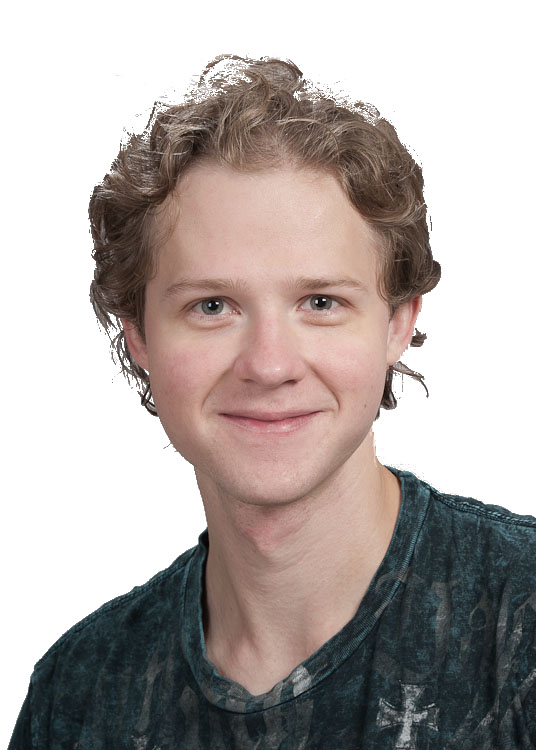
\includegraphics[width=1in,height=1.25in,clip,keepaspectratio]{photos/medley.jpg}}]{J. Kyle Medley}
obtained his BSc in Mechanical Engineering from the University of Missouri-Kansas City and
is currently pursuing a Ph.D. in Bioengineering from the University of Washington, USA.
His research interests include modeling dynamical biophysical processes such as
metabolism and gene expression regulation.
He currently develops libRoadRunner, a software package for simulating dynamical models encoded in SBML.
\end{IEEEbiography}

\begin{IEEEbiography}[{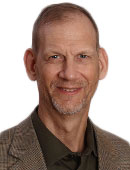
\includegraphics[width=1in,height=1.25in,clip,keepaspectratio]{photos/goldberg.jpg}}]{Arthur P. Goldberg}
received his Ph.D. in Computer Science from the University of California, Los Angeles, USA in 1991 and his A.B. in Astronomy and Astrophysics from Harvard College, USA in 1977. Currently, Dr. Goldberg is an Associate Professor at the Icahn School of Medicine at Mount Sinai, USA. His research focuses on the development of high-performance simulation technologies for WC modeling.
\end{IEEEbiography}

\begin{IEEEbiography}[{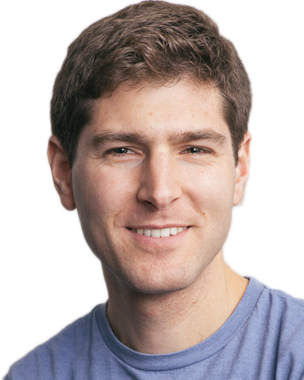
\includegraphics[width=1in,height=1.25in,clip,keepaspectratio]{photos/karr.jpg}}]{Jonathan R. Karr}
received his Ph.D. in Biophysics and M.S. in Medicine from Stanford University, USA in 2014 and his B.S.s in Physics and Brain \& Cognitive Sciences from the Massachusetts Institute of Technology, USA in 2006. Currently, Dr. Karr is a Fellow at the Icahn School of Medicine at Mount Sinai, USA. His research focuses on the development of comprehensive WC computational models and their application to bioengineering and medicine.
\end{IEEEbiography}

\vfill

\end{document}
